\documentclass[12pt]{article}
\usepackage[utf8]{inputenc}
\usepackage[greek,english]{babel}
\usepackage{alphabeta}
\usepackage{fancyhdr}
\usepackage{listings}
\usepackage{mathtools}
\usepackage{xcolor}
\usepackage{float}
\usepackage{siunitx}
\usepackage[margin=0.5in]{geometry}
\usepackage[backend=bibtex]{biblatex}

\lstset {
        basicstyle=\ttfamily,
        columns=fullflexible,
        breaklines=true,
        keepspaces=true,
	showstringspaces=false
}

\title{Εργαστήριο Προηγμένης Αρχιτεκτονικής Υπολογιστών -- Εργασία 2}
\author{Χρήστος Μαργιώλης -- 19390133}
\date{Απρίλιος 2025}

\begin{document}

\begin{titlepage}
        \maketitle
        \begin{figure}[t!]
        \begin{center}
        
\includegraphics[scale=0.3]{./res/uniwalogo.png} \\
        \Large
        \textbf{Πανεπιστήμιο Δυτικής Αττικής} \\
        \large
        Τμήμα Μηχανικών Πληροφορικής και Ηλεκτρονικών Υπολογιστών
        \end{center}
        \end{figure}
\end{titlepage}

\renewcommand{\contentsname}{Περιεχόμενα}
\tableofcontents
\pagebreak

\section{Προσαρμογή προσομοιωτή}

Απενεργοποίηση Enable Forwarding, Enable Target Buffer και Enable Delay Slot:
\\

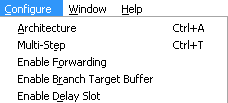
\includegraphics{res/disable.png} \\

Επαλήθευση τιμών παραμέτρων: FP Addition Latency = 4, Multiplier Latency = 7,
Division Latency = 24: \\

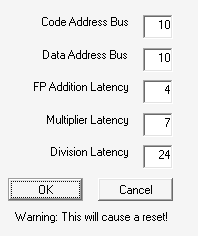
\includegraphics{res/latency.png}

\section{Ερώτημα 1}

Τμήμα Α:

\begin{center}
\begin{tabular}{|l|l|l|l|}
	\hline
	\textbf{Εξαρτώμενη} & \textbf{Αρχική} & \textbf{Εξάρτηση} & \textbf{Από} \\
	\hline
	\lstinline|2 dsub r5,r1,r4| & \lstinline|1 dadd r1,r2,r3| & RAW-A1 & \lstinline|r1| \\
	\hline
	\lstinline|3 or r6,r1,r5| & \lstinline|2 dsub r5,r1,r4| & RAW-A2 & \lstinline|r1, r5| \\
	\hline
	\lstinline|4 dadd r7,r1,r6| & \lstinline|3 or r6,r1,r5| & RAW-A3 & \lstinline|r1, r6| \\
	\hline
\end{tabular}
\end{center}

Τμήμα B:

\begin{center}
\begin{tabular}{|l|l|l|l|}
	\hline
	\textbf{Εξαρτώμενη} & \textbf{Αρχική} & \textbf{Εξάρτηση} & \textbf{Από} \\
	\hline
	\lstinline|2 lw r3,4(r1)| & \lstinline|1 lw r1,0(r2)| & RAW-B1 & \lstinline|r1| \\
	\hline
	\lstinline|4 sw r1,0(r4)| & \lstinline|3 dadd r4,r1,r2| & RAW-B2 & \lstinline|r1| \\
	\hline
\end{tabular}
\end{center}

\section{Ερώτημα 2}

\begin{center}
\begin{tabular}{|l|l|l|}
	\hline
	& \textbf{Τμήμα Α} & \textbf{Τμήμα Β} \\ 	
	\hline
	α) & 6 stalls & 4 stalls \\
	\hline
	β) & Στους κύκλους 3, 4, 6, 7, 9, 10 & Στους κύκλους 3, 4, 7, 8 \\
	\hline
	γ) & & \\
	\hline
	δ) & 15 κύκλοι & 13 κύκλοι \\
	\hline
	ε) & RAW-A1, RAW-A2, RAW-A3 & RAW-B1, RAW-B2 \\
	\hline
\end{tabular}
\end{center}

Τμήμα Α:

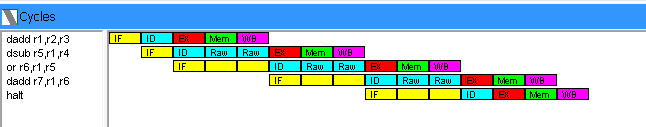
\includegraphics[width=\textwidth]{res/nofwd_p1.png} \\

Τμήμα Β:

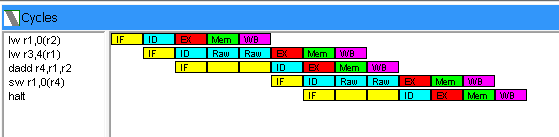
\includegraphics[width=\textwidth]{res/nofwd_p2.png}

\section{Ερώτημα 3}

\begin{center}
\begin{tabular}{|l|l|l|}
	\hline
	& \textbf{Τμήμα Α} & \textbf{Τμήμα Β} \\ 	
	\hline
	α) & 0 stalls & 1 stall \\
	\hline
	β) & Πουθενά & Στον κύκλο 4 \\
	\hline
	γ) &  & \\
	\hline
	δ) & 9 κύκλοι & 10 κύκλοι \\
	\hline
	ε) &  & RAW-B1  \\
	\hline
\end{tabular}
\end{center}

Τμήμα Α:

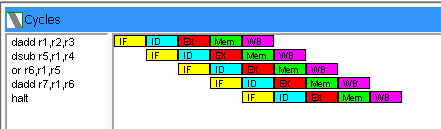
\includegraphics[width=\textwidth]{res/fwd_p1.png} \\

Τμήμα Β:

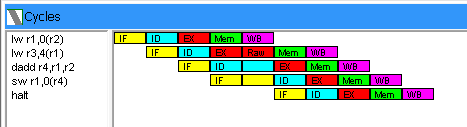
\includegraphics[width=\textwidth]{res/fwd_p2.png}

\section{Ερώτημα 4}

β) Για το τμήμα Α η εκτέλεση επιταχύνθηκε κατά 6 κύκλους, και το τμήμα Β κατά 3
κύκλους.

\end{document}
